\patternThree

\subsection*{Context}

    Graphics constitute a fundamental modality of visual representation for sighted individuals. They are deeply integrated into everyday life, appearing in various forms such as city maps, architectural floor plans, and numerous types of instructional illustrations.

In educational contexts, graphical representations are extensively employed in teaching materials at both school and university levels. These include diagrams, sketches, and technical drawings, which are often created using software tools or produced as freehand illustrations.

    
\subsection*{Problem}

\begin{itshape}

However, non-textual content—such as images, maps, charts, and diagrams—remains largely inaccessible to \ac{bvi} students. This inaccessibility presents a significant barrier to information acquisition and equal participation in educational and professional environments.

\end{itshape}

\subsection*{Solution}

\begin{sol}

Provide textual, tactile, or auditory access to information represented visually in graphics.
  
\end{sol}

In HTML files the so called "alt text"  (alternative text) can give an additional text-based descriptions of visual details of an image. 
Originally intended to give some information if the HTML page is not loaded properly. 
Such descriptions are useful to provide accessible information for people who are visually impaired. This approach can be applied in other formats, too.


Important authoritative regulatory and guideline documents for "alt-text" are  W3C: "Web Content Accessibility Guidelines (WCAG)" \footnote{\url{https://www.w3.org/TR/WCAG21/}}, W3C WAI: “Resources on Alternative Text for Images” \footnote{\url{https://www.w3.org/WAI/alt/}}, W3C WAI: “Understanding Guideline 1.1: Text Alternatives” \footnote{\url{https://www.w3.org/WAI/WCAG22/Understanding/text-alternatives}}, and \ac{uncrpd}: "The Convention on the Rights of Persons with Disabilities"  \footnote{\url{https://social.desa.un.org/issues/disability/crpd/convention-on-the-rights-of-persons-with-disabilities-crpd}}


To make graphics perceivable through touch, they must be converted into raised, tangible structures. 
Color gradients present a significant challenge in this context. Instead, black-and-white graphics composed of lines, contours, and strokes are generally more suitable for tactile representation.

For more complex graphics that include areas beyond simple contours, the first step is to identify the edges of shapes. Many software tools begin this process by converting images into grayscale. Edge detection filters are then applied to extract outlines and essential details. Once the graphic is sufficiently simplified, it can be transformed into a tactile format using raised structures.

Additional information about a graphic can be embedded as metadata. Assistive technologies such as 2D Braille displays can then present this information as text or audio output.

Emerging \ac{ai} technologies are increasingly capable of interpreting and describing graphics. These advancements offer promising solutions for making visual content more accessible to \ac{bvi} students.

One solution for creating raised structures on paper is the use of Swell Touch Paper. This special paper can be printed on using standard printers or written on with a pen. When heat is applied, the printed areas expand, forming raised contours that are easily perceivable by touch.

3D printers have also gained popularity as a tool for producing tactile graphics. They allow for the creation of detailed contours and textures. Educational materials printed in this way are durable and can be reused over extended periods.

Electronic tactile displays, such as 2D Braille displays, provide dynamic tactile feedback. These devices can render static or even animated graphics in real time. They work by precisely raising and lowering an array of pins to create touchable images and patterns.



\subsection*{Examples}


An alternative text for Fig.~\ref{fig:class_diagram}
is generated using a web-site that supports generating alt-text by means of \ac{ai}\footnote{\url{https://barrierefreies.design/werkzeuge/ki-generator-alternativer-text-von-bildern}}.devices. The generated alt-text:
\begin{quoted}
   UML class diagram showing Person superclass with subclasses Student and Lecturer; Student linked to multiple Books with attributes like title and ISBN.
\end{quoted}

Class members were unfortunately suppressed by this tool.

Prompt for chatGPT: "write a alt-text for a html web site describing this diagram". Answer:
\begin{quoted}
UML class diagram showing four classes and their attributes. The classes are Person (attributes: firstname, surname), Student (matriculationNumber, degreeProgram), Lecturer (title, department), and Book (title, ISBN). Student and Lecturer both inherit from Person. There is an association from Person to Book indicating that one person can be linked to many books (1 to n).
\end{quoted}

This description contains the details of the class diagram. 


\textit{PunktBilder} is a software developed at the centre for blind persons (BliZ) at THM.
The \textit{PunktBilder} software is used to create tactile images for \ac{bvi} students at THM. Images are displayed in \textit{PunktBilder} (Fig.~\ref{fig:punktbilder}, ~\ref{fig:punktbilder2}) and can control  2D Braille displays. 

\begin{figure}
    \centering
    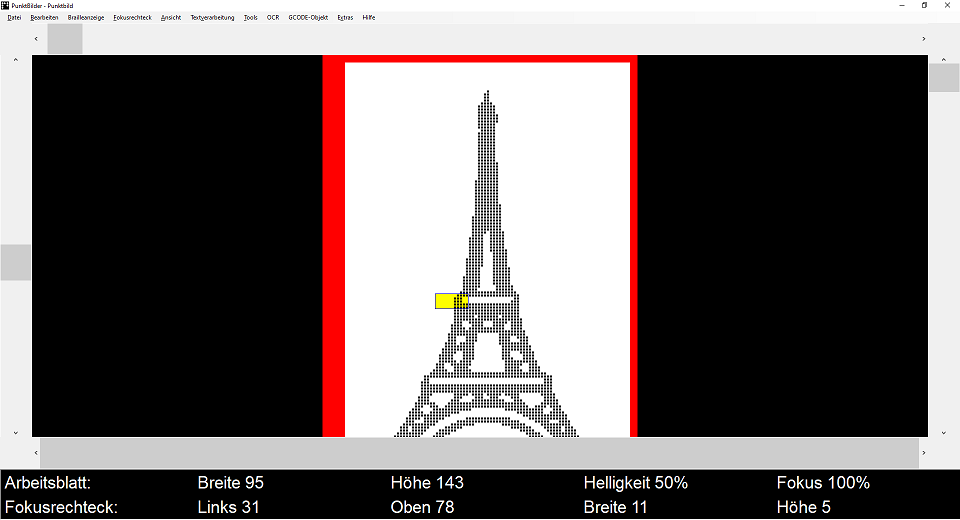
\includegraphics[width=0.7\linewidth]{img/PunktBilder.png}
    \caption{Screenshot from the \textit{PunktBilder} application (Source: THM / BliZ)}
    \label{fig:punktbilder}
\end{figure}

\begin{figure*}[ht!]
    \centering
    \begin{subfigure}[t]{0.5\textwidth}
        \centering
        
\includegraphics[width=.5\linewidth]{img/THM_Pattern.pdf}
      
    \end{subfigure}%
    \begin{subfigure}[t]{0.5\textwidth}
        \centering
        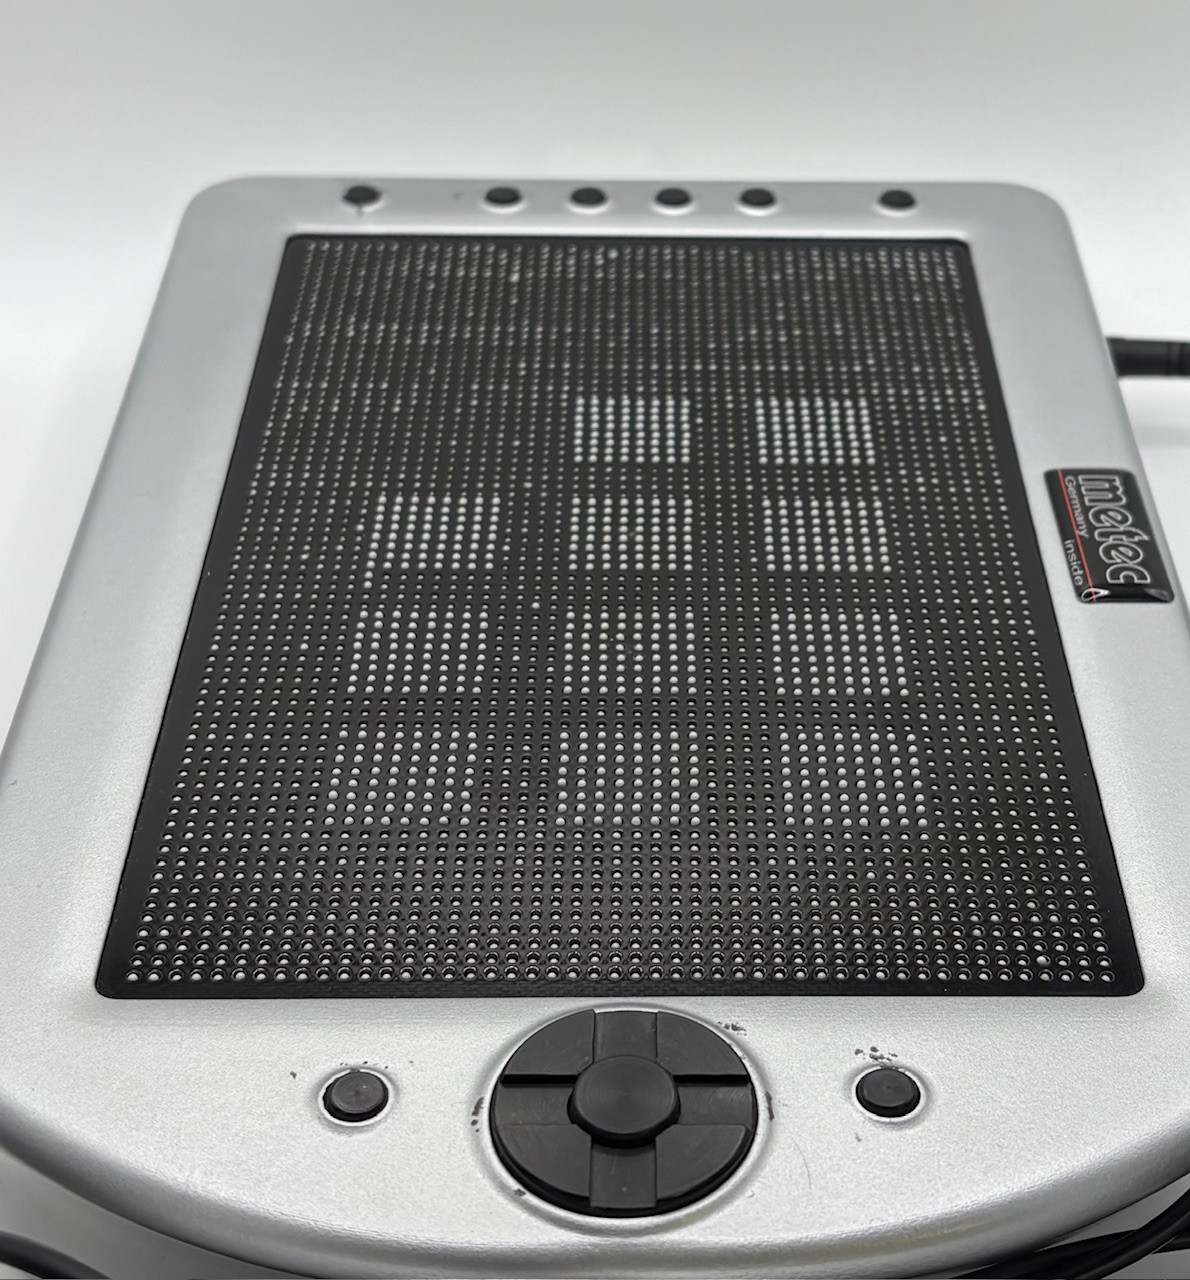
\includegraphics[width=.5\linewidth]{img/PunktBilder-BliZ.jpg}       
    \end{subfigure}
    \caption{Dot pattern for the logo of the THM (left), converted with \textit{PunktBilder} for a 2D Braille display (right) (Source: THM / BliZ)}
    \label{fig:punktbilder2}
\end{figure*}


\subsection*{Consequences}

% Benefits
\renewcommand{\labelenumi}{$+$}
\begin{enumerate}
\item Multi-modal accessibility is achieved by making textual explanations of graphics accessible using assistive technology. 

\item Generative AI can take over the creation of textual descriptions of graphics for authors.

\item The use of ‘alt text’ in HTML documents better fulfills regulatory requirements for accessibility. 


\end{enumerate}

% Liabilities
\renewcommand{\labelenumi}{$-$}
\begin{enumerate}
\item The manual creation of textual descriptions of graphics is time-consuming, and consideration must be given to which aspects and content of a graphic are significant.

\item The automatic generation of textual descriptions Generative AI should be checked by authors for content accuracy.

\item Devices for the production of tactile output formats such as 3D printers or thermal printers are expensive and complex to use.

\item Devices for dynamically changeable tactile outputs are expensive and require special software to control them. 
\end{enumerate}

 
\subsection*{Related Work}

Non-profit organizations like \textit{ProBlind}\footnote{\url{https://www.problind.org/en/}} are actively working to improve access to graphics for blind and visually impaired individuals. As part of a global community initiative, they are developing a free online database of tactile graphics, accessible worldwide. They have developed a tool chain to convert graphics into tactile graphics, as shown in Fig.~\ref{fig:problind}.

\begin{figure}[ht]
    \centering
    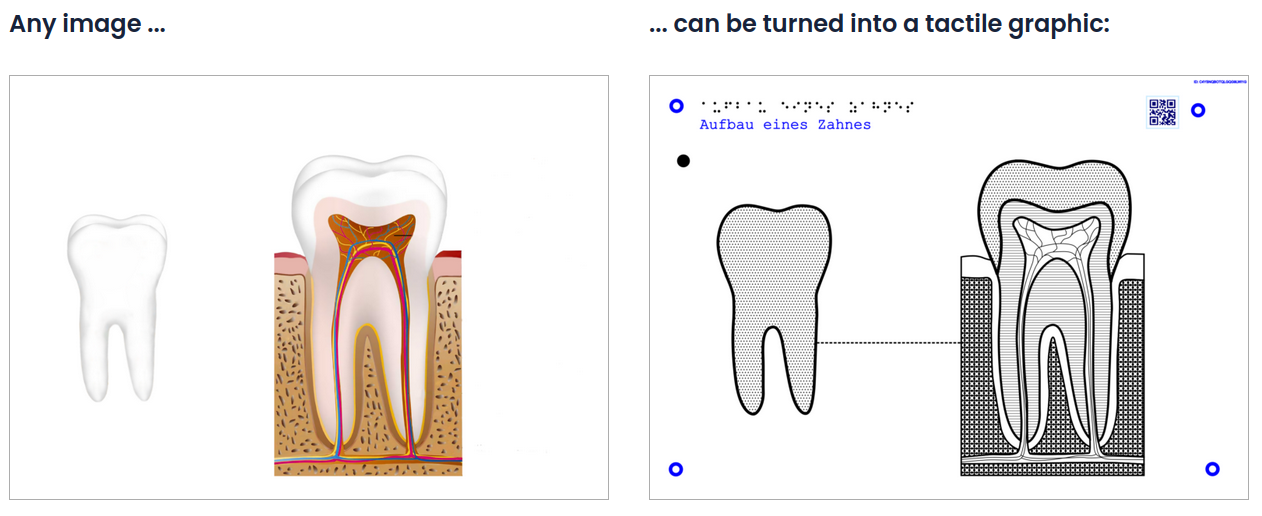
\includegraphics[width=.8\linewidth]{img/problind.png}
    \caption{Generation of tactile graphics (Screenshot from \texttt{www.problind.org})}
    \label{fig:problind}
\end{figure}

Many other schools for the blind and organizations that support the blind and visually impaired provide libraries of graphics that can be printed as tactile graphics.


In \cite{pissaloux2022} 
the accessibility challenges faced by visually impaired people  in interpreting graphical data, such as images and maps, is addressed. Their solution introduces the concept of a tactile gist as a simplified, touch-based representation of essential visual information. Based on experiments with VIP participants, the study establishes new design rules for 2D tactile representations using two mediums: thermo-formed paper and a force-feedback tablet called F2T.

In \cite{gay2021} this Force-Feedback Tablet (F2T) is introduced. The F2T’s architecture is based on a flat thumb-stick mounted on a 2D actuated support, enabling force feedback effects on user’s finger.


In \cite{ducasse2018} the challenge of accessibility of maps is addressed. The authors pointed out, that mobility and orientation are major challenges for visually impaired individuals. Primarily because verbal descriptions and GPS systems do not effectively convey spatial layouts. Unlike sighted individuals who rely on visual perception or maps, visually impaired people face limited access to geographical maps, which significantly impacts their mobility. The authors review various accessible interactive map solutions developed for visually impaired users, including a range of prototypes such as 3D-printed maps and devices with dynamically actuated structures.